\chapter{Resumen}
El objetivo del proyecto es crear un bot que sea capaz de poder gestionar el aforo de un espacio público (gimnasios, tiendas, supermercados, etc)
El bot estará desarrollado en Python, será desplegado en la red de Telegram y tendrá una comunicación con un backend propio que también será desarrollado en Python. 
Se simularán los dispositivos hardware de tornos / cámaras y detección de personas con un programa Python para llevará el conteo del aforo e inundará de información de aforo a todo el backend productivo.
Gracias a este backend productivo el bot será entrenado y será capaz de tomar decisiones productivas, resultando de gran utilidad para el usuario.

\begin{center}
    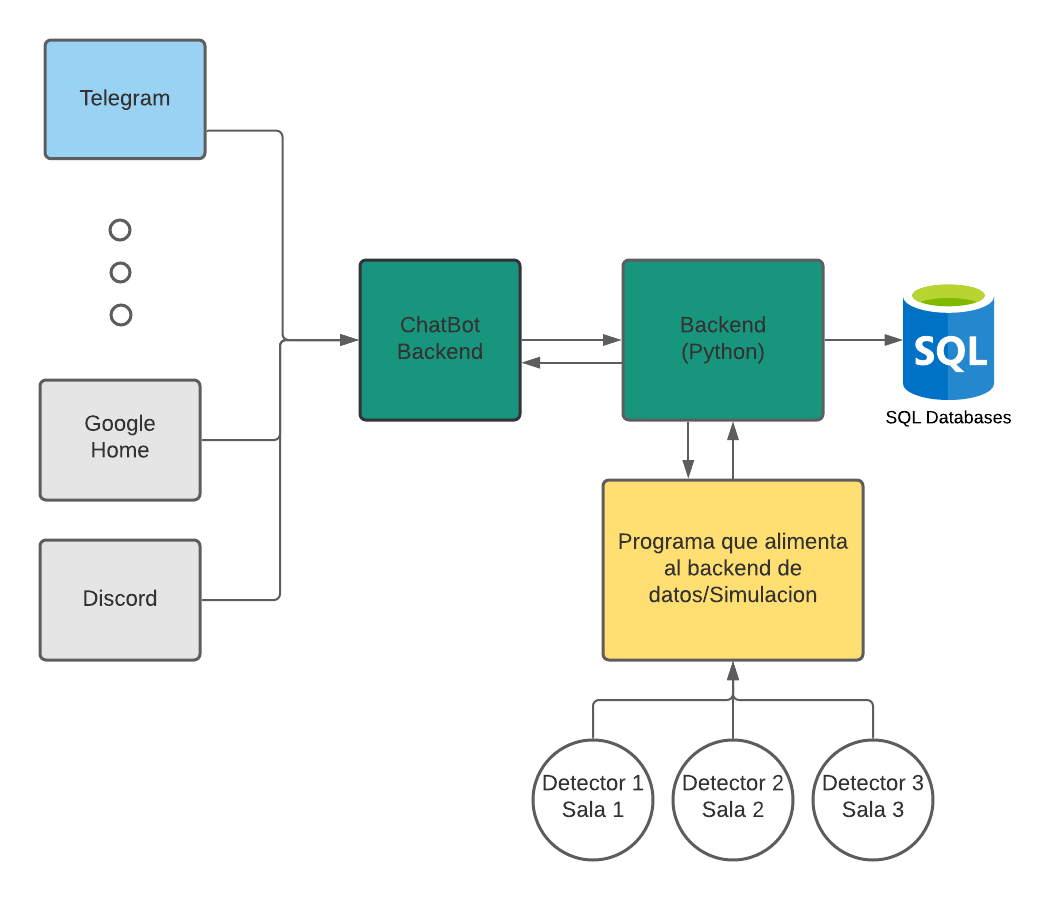
\includegraphics[scale=0.25]{imagenes/dig1/dig1.png}
\end{center}

\chapter{Abstract}
<<Abstract of the Final Degree Project. Maximum length: 2 pages.>>

%%%%%%%%%%%%%%%%%%%%%%%%%%%%%%%%%%%%%%%%%%%%%%%%%%%%%%%%%%%
%% Final del resumen. 
%%%%%%%%%%%%%%%%%%%%%%%%%%%%%%%%%%%%%%%%%%%%%%%%%%%%%%%%%%%